\section{Introduction}
\label{sec:introduction}
\FloatBarrier % Now figures cannot float above section title
This section should concentrate on what has previously been done in the field of research, so that it incentivizes the experiment. Why is there a need to gain knowledge on this specific field, and what motivates you to conduct the experiment? Often the introduction lists up a lot of historical facts and previous reports, and then it presents the topic for the report. The section is here for make a smooth transaction over to what you will be covering later on. It may be a good idea to present figures to back up your claims as done in figure \ref{fig:intro_co2}. Never post jpg, jpeg or bmp files in figures, but try to stick to png or eps format. Even though you have presented the figure in this text, the caption on the figure must still be able to present the information alone independent of this text! It should also be placed BENEATH the actual figure. Also remember to always write passive, i.e no personal pronouns (I, you, he, we, you, they). It is recommended that you learn Mendeley for managing your references that has great support in Sharelatex. Upper left corner $\rightarrow$ Menu $\rightarrow$ Mendeley inserts your whole personal library into the document, so that you don't have to worry about formatting your references correctly. \LaTeX does that for you.
% Historical chart of CO2 emissions
\begin{figure}[htb] % Here, top, bottom priority list
    \centering
    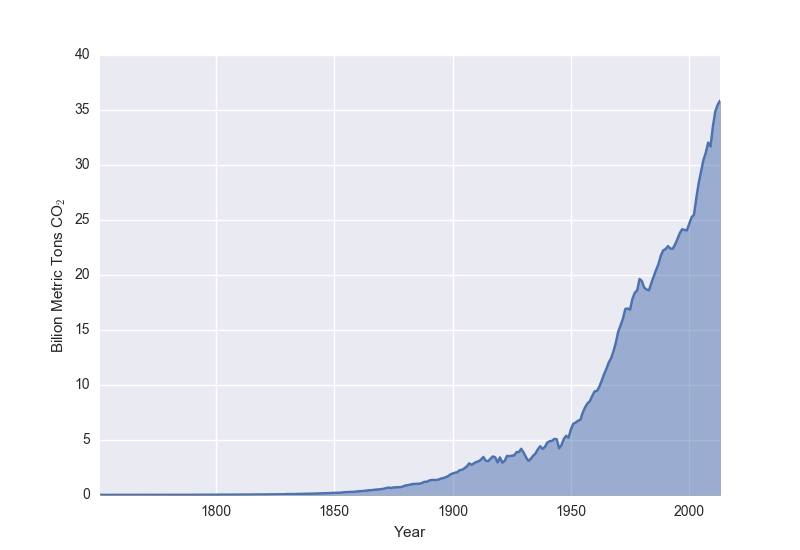
\includegraphics[scale=0.45]{Introduction/figures/Historic_CO2_Emission}
    \caption{This text should be able to stand alone independent of text outside figure!}
    \label{fig:intro_co2}
\end{figure}